\section{Fazit}
\label{sec:fazit}
Auf den ersten Blick scheint die Bandbreite mit der Größe der komprimierten Daten zu korrelieren.
Wie in den Ergebnissen zu sehen, bietet die Quantisierung dazu noch eine nicht zu verachtende Reduktion der Speichergröße.
Die Kombination aus Quantisierung und der anschließenden Kompression mit Brotli-G scheint dazu noch bessere Kompressionsverhältnisse zu liefern. \newline
Die Ergebnisse aus Kap.~\ref{sec:ergebnisse} sollen zuletzt bewertet und analysiert werden.
Die Bewertungsmaße liegen bei den Kompressionsverhältnissen und der Bandbreite.

\subsection{Analyse der Dekompressionszeit und Bandbreite}
\label{subsec:ana_bandwidth}
Eine Möglichkeit für die geringe Bandbreite scheint auf den ersten Blick die Größe der komprimierten Daten zu sein.
Auffällig ist nämlich die geringe Bandbreite bei kleinen Dreiecksnetzen wie der Fandisk.
Mit einer komprimierten Größe von 0,160 MB benötigt diese am wenigsten Speicherplatz, und erreicht eine Bandbreite von \textit{0,054 GiB/s}.
Weitere Beispiele sind das Bunny mit einer Größe von \textit{1,067 MB} und einer Bandbreite von \textit{0,503 GiB/s}, der Dinosaur mit 1,713 MB und einer Bandbreite von 0,825 GiB/s und der Rockerarm mit 1,139 MB und einer Bandbreite von \textit{0,399 GiB/s}.
Es scheint dabei zudem eine untere Grenze der Dekompressionszeit zu geben.
Diese liegt bei den sehr kleinen Dreiecksnetzen bei \textit{2 ms - 3 ms}.
Bei Betrachtung der mittelgroßen Dreiecksnetze des Datensatzes scheint die Dekompressionszeit jedoch nicht wie erwartet zuzunehmen.
Die Dekompressionszeit der Igea, des Armadillo und des Angels beträgt ebenfalls jeweils \textit{3 ms}.
Die Größe der komprimierten Dreiecksnetze liegt bei \textit{4,033 MB, 4,486 MB und 7,239 MB}.
So sind diese ca. 3 - 4 mal so groß wie die kleinen Dreiecksnetze. 
Bei einer höheren Dateigröße und gleichbleibender Dekompressionszeit steigt natürlich die Bandbreite. 
Die Bandbreite der Igea liegt bei \textit{1,473 GiB/s}, des Armadillos bei \textit{1,415 GiB/s} und der des Angels bei \textit{2,346 GiB/s}.
Die Ergebnisse sind zwar besser, aber dennoch noch nicht auf einem hohen Niveau. \newline

Eine mögliche Erklärung für diese untere Schranke kann die Zeitrechnung des Brotli-G Dekodierers sein.
Die Zeitrechnung des Brotli-G Dekodierers misst nicht ausschließlich die Dauer des Compute Shaders.
Der Umstand einer unteren Schranke bei 2 ms kann am Overhead der API-Aufrufe von DirectX12 liegen.
Die Zeitrechnung beginnt demnach bei dem Aufruf der decodeGPU Methode und endet, nachdem der Destruktor der Klasse das Objekt zerstört, das den Compute Shader mit Daten gefüttert und ausgeführt hat. \newline

Die Ergebnisse der zwei größten Dreiecksnetze des Datensatzes scheinen die These zu stützen, dass die kleinen Dreiecksnetze nicht effektiv von Brotli-G verarbeitet werden oder ein zu großer prozentualer Anteil an Overhead das Ergebnis verfälscht.
Die Hand erreicht eine Bandbreite von \textit{2,218 GiB/s} bei einer komprimierten Größe von \textit{8,195 MB}.
Bezüglich der Bandbreite erreicht der Welsh Dragon \textit{4,192 GiB/s}, mit einer komprimierten Größe von \textit{31,717 MB}.
Auch hier scheint die Korrelation von komprimierter Größe und Bandbreite weiterzubestehen.

\subsection{Analyse der Kompressionsverhältnisse}
\label{subsec:ana_ratios}
Die Kompressionsverhältnisse, die nur mittels Brotli-G erzielt wurden, sind gut.
Bei dem Datensatz ergibt sich ein durchschnittliches Kompressionsverhältnis von \textit{1,99} über alle Dreiecksnetze verteilt.
Das größte Kompressionsverhältnis verzeichnet die Fandisk mit \textit{2,29}, während das Horse das geringste Kompressionsverhältnis von \textit{1,84} besitzt.
Bei den Kompressionsverhältnissen gibt es keine Überraschungen oder Auffälligkeiten wie bei der Bandbreite.

\subsection{Analyse der quantisierten Dreiecksnetze}
\label{subsec:ana_quantized}
Der Großteil der Daten eines Dreiecksnetzes besteht aus seiner Geometrie \cite{Jakob2017}.
Bei Betrachtung der Komponenten ist zwar erkennbar, das es wesentlich mehr Dreiecke, und somit auch mehr Indizes, als Vertices gibt.
Wenn als Topologie eine \textit{Triangle List} verwendet wird, gelangt man auf ein Verhältnis von 
\begin{equation*}
V:T = 1:2
\end{equation*}
Da ein Dreieck aus 3 Indizes besteht, enthält ein Dreiecksnetz von dieser Topologie in etwa 6 Indizes pro Vertex (Euler's Formel) \cite{Engstad2011}.
Angenommen, ein Vertex bestehe lediglich aus Positionen und Normalen, wie es bei dem verwendeten Datensatz dieser Arbeit der Fall ist.
So enthält ein Vertex ohne Kompression der Daten
\begin{equation*}
3 \cdot 4 \ \text{Byte} = 12 \ \text{Byte}
\end{equation*}
Gleitkommazahlen für die Position im 3-dimensionalen Raum.
Und nochmal so viele Byte für die Normalen.
Da gib dem Vertex eine Größe aus 24 Byte.
Ein unkomprimierter Index wird in einem Integer ohne Vorzeichen gespeichert, der 4 Byte beansprucht \cite{Microsoft2021a}. \newline
Beachtet man das Verhältnis der Euler Formel bei Dreiecksnetzen, enthalten 6 Indizes mit 192 Bit die gleiche Datenmenge wie ein Vertex mit Position und Normale.
Zu beachten ist jedoch, dass neben der Position auch Texturkoordinaten, Farben, Tangenten und Bitangenten in den Vertex Attributen vorhanden sein können. \newline
Jedenfalls ist erkennbar, dass die Vertices einen maßgeblichen Einfluss auf die Datengröße nehmen.
Bei jedem einzelnen Dreiecksnetz des Datensatzes ist eine Reduktion der Daten von \textit{28,4 \%} zu sehen.
Die Quantisierung mindert jedoch nicht nur die originalen Eingabedaten.
Vergleicht man die von Brotli-G komprimierten Originaldaten und die von Brotli-G komprimierten Daten seines quantisierten Gegenübers, so ist eine Reduktion der komprimierten Daten von durchschnittlich \textit{39,71 \%} möglich.
Die meisten Dreiecksnetze sind in einem Bereich von \textit{38 \% - 42 \%}.
Die Ausreißer liegen jedoch nicht weit entfernt von diesem Bereich, mit dem Armadillo der mit \textit{32,6 \%} am schlechtesten abgeschnitten hat, während der Welsh Dragon mit \textit{45,6 \%} die größte Reduktion der Originaldaten hat.
Diese Diskrepanz der Prozente ist gut erkennbar, wenn die Kompressionsverhältnisse von quantisierten und nicht quantisierten Dreiecksnetzen betrachtet werden.
Hier wird schnell klar, das der Armadillo mit \textit{6,42 \%} den geringsten Zuwachs der Kompressionsverhältnisse erlangt hat, während der Welsh Dragon mit \textit{32,5 \%} den besten Zuwachs der Kompressionsverhältnisse verzeichnet.
Diese komprimierten Daten können direkt aus einem Speichermedium in den GPU-RAM hochgeladen werden, wo sie vom Brotli-G Compute Shader dekomprimiert und vom Mesh Shader gerendert werden. \newline

Das verbesserte Kompressionsverhältnis stammt von dem losgewordenen Rauschen der Originaldaten.
Die Daten des Dreiecksnetzes werden für gewöhnlich in einer Genauigkeit repräsentiert, die für die Darstellung einfacher 3D-Modelle nicht benötigt wird.
Wenn diese richtig quantisiert werden, ist der Verlust an visueller Qualität meist so gering, das diese kaum auffällt.
Die Fließkommazahl ist somit frei von Signalrauschen, das sehr schwer zu kodieren ist, da diese Zeichenfolgen oft zufällig oder willkürlich sind.
\begin{figure}[htb]
  \centering  
  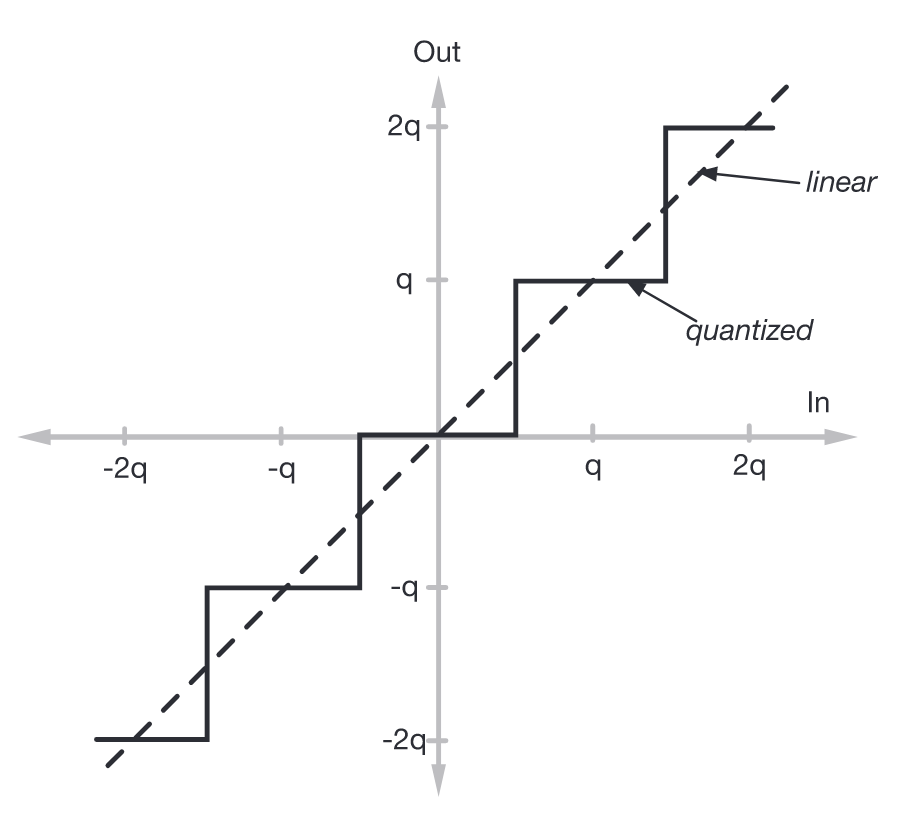
\includegraphics[scale=0.35]{Bilder/quantization.png}
  \caption[Mid-Tread Quantisierer]{\textbf{Mid-Tread Quantisierer} Die Abbildung zeigt eine Gegenüberstellung von den möglichen Werten vor der Quantisierung (gestrichelte Linie) und den möglichen Werten nach der Quantisierung (durchgezogene Linie.
  Die Abbildung stammt aus \cite{Bennett2020} }
  \label{fig:mid-tread_quantizer}
\end{figure}

\subsection{Ausblick für spätere Arbeiten}
\label{subsec:ausblick}
Wie zu sehen ist, ergeben sich durch die Komprimierung mittels Brotli-G gute Kompressionsverhältnisse.
Die Auswertung der Ergebnisse zeigt auch, dass weitere Verfahren zur Datenkompression nicht nur zu einer direkten Datenreduktion führen, sondern auch die Ergebnisse von Brotli-G verbessern können.
In dieser Arbeit wurde der Einsatz von der Quantisierung verwendet.
Weitere Verfahren, die in Kombination mit Brotli-G getestet werden können, sind die \textit{prädiktive Kodierung}, \textit{Triangle Traversal Encoding} oder \textit{Connectivity Compression} \cite{Jakob2017}.
Da sich die Indizes lediglich in einem bestimmten kleinen Intervall bei der Verwendung von Meshlets befinden, würde sich zusätzlich anbieten, diese nicht einzeln in einer 4 Byte Datenstruktur wie einem Integer zu speichern, sondern jeweils drei Indizes (bei einer Triangle List eine Primitive) in einen Integer zu packen. \newline

Nach einem Blogpost auf GPUOpen von AMD wurde die Version 1.1 von Brotli-G mit dem Compressonator Version 4.5 veröffentlicht.
Die Tests die in dem Blogpost behandelt werden, richten sich zwar an Texturen, die Ergebnisse von der neuen Version von Brotli-G sind dennoch sehenswert.
Im Vergleich zur alten Version reduziert der Compressonator mit der neuen Brotli-G Version die komprimierten Texturen im Durchschnitt um weitere \textit{10 \% - 15 \%}, in besonders guten Fällen sogar um \textit{20 \%} \cite{Levesque2024}.
Die Brotli-G Version 1.1 wurde leider erst gegen Ende dieser Arbeit veröffentlicht, wodurch die vorliegenden Ergebnisse auf der Version 1.0 bestehen.
Die besseren Ergebnisse des Compressonators lassen auf zukünftig bessere Resultate und vor allem auf eine effektivere Ausnutzung der Bandbreite des PCIe-Busses hoffen.
Die Ergebnisse dieser Arbeit in der Hinsicht der Dekompressionszeit und Bandbreitenausnutzung sind selbst bei den größeren Dreiecksnetzen weit von gewünschten Werten entfernt.
Für die Versuche wurde die Grafikkarte \textit{Radeon RX 6650 XT} von AMD verwendet.
Diese soll laut Datenbankeintrag eine maximale Bandbreite von \textit{280 GB/s}, also zum Vergleich umgerechnet ungefähr \textit{260 GiB/s} erreichen.
Es ist zwar unwahrscheinlich, an dieses Maximum zu gelangen, dennoch wäre eine bessere Ausnutzung der Bandbreite wünschenswert. \newpage
\begin{figure}[htb]
  \centering  
  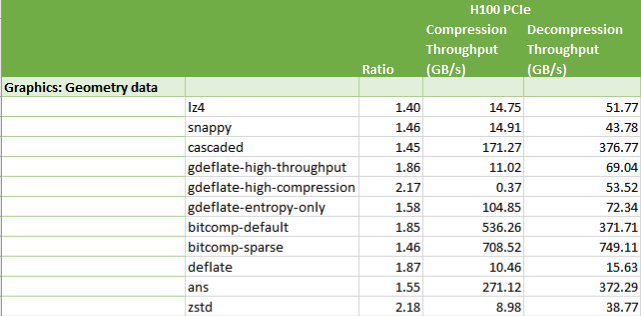
\includegraphics[scale=0.70]{Bilder/nvComp_geometry_results.png}
  \caption[NVIDIAs nvCOMP Testergebnisse]{\textbf{NVIDIAs nvCOMP Testergebnisse} In der Abbildung sind die Ergebnisse der NVIDIA Bibliothek nvCOMP zu sehen, die verlustfreie Datenkompression und Dekompression unter Verwendung einer GPU ausführt.
  Die Abbildung ist von NVIDIAs öffentlicher Developer Website. https://developer.nvidia.com/nvcomp }
  \label{fig:nvCOMP}
\end{figure}
In der Abbildung.~\ref{fig:nvCOMP} ist zu sehen. welche Kompressionsverhältnisse unterschiedliche Algorithmen der nvCOMP Bibliothek.
Neben dieser sind die Bandbreiten der Kompression und Dekompression.
Das Ziel ist es nicht, die Bandbreiten dieser Arbeit mit den Ergebnissen von nvCOMP zu vergleichen.
Dabei spielt auch nicht nur der verwendete Datensatz eine Rolle.
Die verwendete GPU aus Abbildung~\ref{fig:nvCOMP} ist nicht für Privatpersonen gebaut worden.
Vor allem ist die \textit{Tensor Core GPU} H100 für Unternehmen gedacht, die GPUs für aufwendige Rechenarbeiten benötigen.
Dementsprechend erzielt diese sehr viel bessere Ergebnisse, als die für Privatpersonen geeignete RX 6650 XT.
Dennoch kann aus dieser Abbildung entnommen werden, das eine sehr viel höhere Bandbreite erzielt werden kann, als es in dieser Arbeit der Fall war.

